\documentclass[12pt, a4]{article}
\usepackage[margin=2cm]{geometry}
\setlength{\textfloatsep}{10pt plus 0pt minus 0pt}
\setlength{\floatsep}{10pt plus 0pt minus 0pt}
\setlength{\intextsep}{10pt plus 2pt minus 2pt}

\usepackage{parskip}
\usepackage{hyperref}
\usepackage{nameref}
\usepackage{enumitem}

\usepackage{amsmath}
\usepackage{amssymb}

\usepackage{fancyhdr}
\usepackage{titling}

\usepackage{pgfplots}
\pgfplotsset{compat=1.16}

\usetikzlibrary{decorations.pathreplacing}

\author{Pascal Lüscher}
\title{Mathematical Optimization – Problem set 1}

\pagestyle{fancy}
\fancyhf{}
\rhead{
	\thetitle\\
	\theauthor
}

\rfoot{
	Page: \thepage
}


\begin{document}
\paragraph{Problem 1: Graphical solution of a linear program}

\begin{equation*}
	\begin{array}{lcrcrcr}
		\text{max} &  &  &  & x_2 &  & \\
		\text{s.t} & - & 4x_1 & - & x_2 & \leq & -8\\
		& - & x_1 & + & x_2 & \leq & 3\\
		&&& - & x_2 & \leq & -2 \\
		&& 2 x_1 & + & x_2 & \leq & 12 \\
		&& x_1 &&&\geq&0\\
		&& &&x_2&\geq&0
	\end{array}
\end{equation*}

\newcommand{\lightgray}{black!30}
\newcommand{\addPlotLDown}[1]{
	\addplot[mark=none, domain=-1:9, color=\lightgray,
		decoration={border,segment length=1mm,amplitude=1.5mm,angle=-135},
		postaction={decorate}
	] {#1};
	\addplot[mark=none, domain=-1:9] {#1};
}
\newcommand{\addPlotRUp}[1]{
	\addplot[mark=none, domain=-1:9, color=\lightgray,
		decoration={border,segment length=1mm,amplitude=1.5mm,angle=135},
		postaction={decorate}
	] {#1};
	\addplot[mark=none, domain=-1:9] {#1};
}

\subparagraph{a}\label{pg:a} \textit{Determine all optimal solutions graphically.}

\begin{figure}[ht]
	\centering
	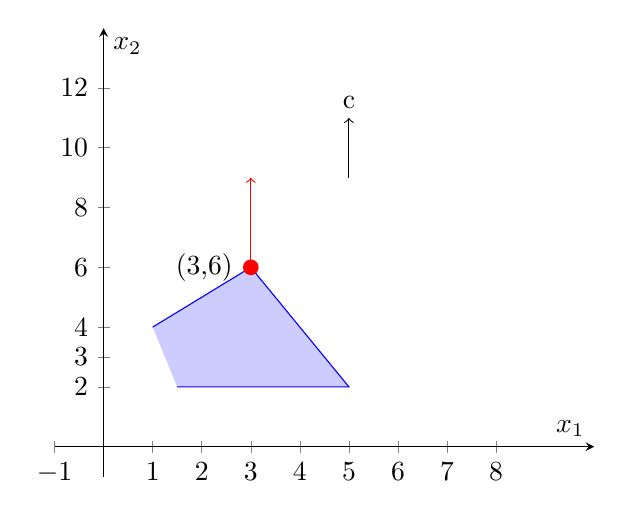
\begin{tikzpicture}
		\begin{axis}[
			axis x line=center,
			axis y line=center,
			xlabel=$x_1$,
			ylabel=$x_2$,
			xmin=-1,
			ymin=-1,
			xmax=10,
			ymax=14,
			xtick={-1,0,1,2,...,8},
			ytick={0,2,3,4,6,8,10,12}
		]
		
		\addplot[fill=blue!20,draw=none]coordinates{(1,4)(3,6)(5,2)(1.5,2)};

		\addPlotRUp{-4*x + 8};
		\addPlotLDown {x+3}
		\addPlotRUp{2}
		\addPlotLDown{-2*x+12}

		\addplot[fill=none,draw=blue]coordinates{(1,4)(3,6)(5,2)(1.5,2)};
		\draw[red, ->](3,6)--(3,9);
		\node[label={180:{(3,6)}}, circle, fill=red, inner sep=2pt] at (axis cs:3,6) {};
		
		\draw[black, ->](5,9)--(5,11);
		\coordinate[label=c] (c) at (5,11);
		\end{axis}
	\end{tikzpicture}
\end{figure}

\subparagraph{b}{\label{pg:b} \textit{Instead of maximizing the objective function, minimize it and graphically determine all optimal solutions of the minimization problem.}}

\begin{figure}[ht]
	\centering
	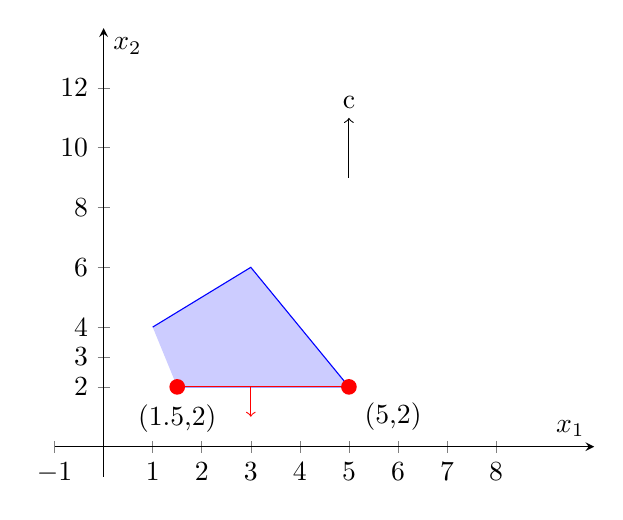
\begin{tikzpicture}
		\begin{axis}[
			axis x line=center,
			axis y line=center,
			xlabel=$x_1$,
			ylabel=$x_2$,
			xmin=-1,
			ymin=-1,
			xmax=10,
			ymax=14,
			xtick={-1,0,1,2,...,8},
			ytick={0,2,3,4,6,8,10,12}
			]
		
			\addplot[fill=blue!20,draw=none]coordinates{(1,4)(3,6)(5,2)(1.5,2)};
			\addPlotRUp{-4*x + 8};
			\addPlotLDown {x+3}
			\addPlotRUp{2}
			\addPlotLDown{-2*x+12}
		
			\addplot[fill=none,draw=blue]coordinates{(1,4)(3,6)(5,2)(1.5,2)};
			\draw[red](1.5,2)--(5,2);
			\node[label={270:{(1.5,2)}}, circle, fill=red, inner sep=2pt] at (axis cs:1.5,2) {};
			\node[label={-45:{(5,2)}}, circle, fill=red, inner sep=2pt] at (axis cs:5,2) {};
			\draw[red, ->](3,2)--(3,1);
			
			
			\draw[black, ->](5,9)--(5,11);
			\coordinate[label=c] (c) at (5,11);
		\end{axis}
	\end{tikzpicture}
\end{figure}

\subparagraph{c}\label{pg:c} \textit{Change the fourth constraint $2x_1 + x_2 \leq 12$ such that
\begin{enumerate}[itemindent=30pt,label=(\roman*)]
	\item the point (5, 2) still satisfies the fourth constraint with equality, and
	\item the maximization problem becomes unbounded.
\end{enumerate}
}
A simple change would be to make the constraint unnecessary by changing $\leq$ to $\geq$. The maximization problem becomes unbounded since there is always an improved maximum value ($\infty$).


\begin{figure}[ht]
	\centering
	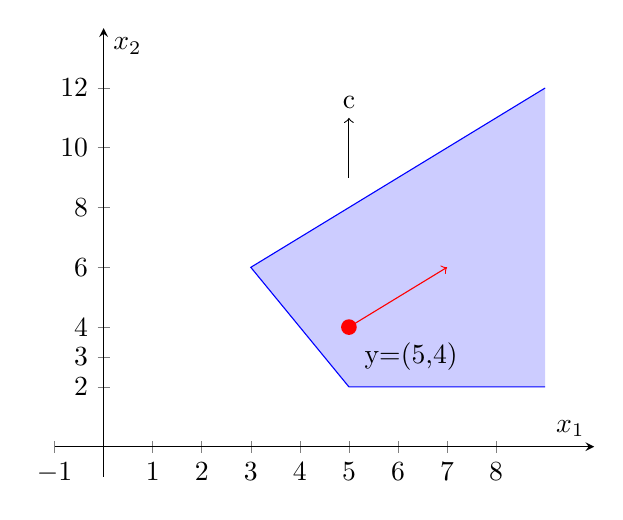
\begin{tikzpicture}
		\begin{axis}[
			axis x line=center,
			axis y line=center,
			xlabel=$x_1$,
			ylabel=$x_2$,
			xmin=-1,
			ymin=-1,
			xmax=10,
			ymax=14,
			xtick={-1,0,1,2,...,8},
			ytick={0,2,3,4,6,8,10,12}
			]
			
		\addplot[fill=blue!20,draw=none]coordinates{(3,6)(9,12)(9,2)(5,2)};

		\addPlotRUp{-4*x + 8};
		\addPlotLDown {x+3}
		\addPlotRUp{2}
		\addPlotRUp{-2*x+12}
		
		\addplot[fill=none,draw=blue]coordinates{(9,12)(3,6)(5,2)(9,2)};
		\draw[black, ->](5,9)--(5,11);
		\coordinate[label=c] (c) at (5,11);
		\draw[red, ->] (5,4) -- (7,6);
		\node[label={-45:{y=(5,4)}}, circle, fill=red, inner sep=2pt] at (axis cs:5,4) {};
			
		\end{axis}
	\end{tikzpicture}
\end{figure}

\subparagraph{d}\label{pg:d} \textit{Change the right-hand side of the fourth constraint $2x_1 + x_2 \leq 12$ (i.e., the number $12$) such
that the maximization problem becomes infeasible. Is the corresponding minimization problem
infeasible, as well?}

Any value $< 5$ will do, the min. problem will become infeasible too since there is no polyhedron.
\begin{figure}[ht]
	\centering
	\begin{tikzpicture}
		\begin{axis}[
			axis x line=center,
			axis y line=center,
			xlabel=$x_1$,
			ylabel=$x_2$,
			xmin=-1,
			ymin=-1,
			xmax=10,
			ymax=14,
			xtick={-1,0,1,2,...,8},
			ytick={0,2,3,4,6,8,10,12}
			]		
			\addPlotRUp{-4*x + 8}
			\addPlotLDown{x+3}
			\addPlotRUp{2}
			\addPlotLDown{-2*x+4}
			
			\draw[black, ->](5,9)--(5,11);
			\coordinate[label=c] (c) at (5,11);
		\end{axis}
	\end{tikzpicture}
\end{figure}
\subparagraph{e} \textit{Prove that the linear programs that you wrote in parts (c) and (d) are unbounded and infeasible,
respectively. How would you prove optimality of the solutions you found in parts (a) and (b)?}

\begin{enumerate}
	\item unbounded: certificate of unboundedness: there is no constraint limiting $x_2$ from growing. $y = (5,4)$, $q = \begin{pmatrix}
		-1\\ 
		1
	\end{pmatrix}$.
	\item infeasible: if there is no polyhedron, there cannot be a solution.
	\item optimality in a and : Introducing the constraint $x_2 \geq 6$  which is perpendicular to the objective reduces the polyhedron to a vertex. Therefore the dimension dropped to 0 and the unique optimum is found.
	\item optimality in b: introducing the constraint $x_2 \leq 2$ which is perpendicular to the objective results in a 1-dimensional edge. Therefore the dimension dropped and the minimum is found.		
\end{enumerate}
\end{document}